\documentclass[11pt]{article}
\usepackage[utf8]{inputenc}
\usepackage[russian]{babel}
\usepackage{amssymb}
\usepackage{amsmath}
\usepackage{graphicx}
\usepackage{subcaption}
\graphicspath{ {./images/} }

\let\oldemptyset\emptyset
\let\emptyset\varnothing

\begin{document}
        \begin{center}
        Вариант 7
        \end{center}

        \textit{\textbf{Задание 1}}

        \textit{Универсальное множество состоит из 26 строчных букв латинского
алфавита. Заданы множества A, B, C и D. Вычислить мощность множеств X
и Y.}

\textit{Даны множества
$A=\{b,f,g,m,o\}, B=\{b,g,h,l,u\}, C=\{e,f,m\}, D=\{e,g,l,p,q,u,v\}$\\
Вычислить мощность множеств}
$$X = (A \setminus C) \cup (B \cap C),
Y=(A \cap \bar B) \cup (D \setminus C) $$

\underline{Решение:}

1. Определим элементы множества 
$X = (A \setminus C) \cup (B \cap C)$.

Для этого найдём сначала разность множеств $A \setminus C$.
Для этого вычеркнем из множества $A=\{b,f,g,m,o\}$ элементы
$\{f, m\}$, принадлежащие $C=\{e,f,m\}$. Следовательно,
$A \setminus C = \{b, g, o\}$.
Затем найдём пересечение множеств $B \cap C$.
Множества $B$ и $C$ не имеют общих элементов. Следовательно,
$B \cap C = \emptyset$.
Таким образом, объединение $(A \setminus C) \cup (B \cap C)$ состоит из
трёх элементов $\{b, g, o\}$.

Мощность множества 
$X = (A \setminus C) \cup (B \cap C)$ равна 3.

2. Определим элементы множества 
$Y=(A \cap \bar B) \cup (D \setminus C)$

Найдем дополнение B . Универсальное множество по условию задания
состоит их 26 букв
$\{a,b,c,d,e,f,g,h,i,j,k,l,m,n,o,p,q,r,s,t,u,v,w,x,y,z\}$.
Если отсюда исключить 5 элементов множества $B$, то получим множество
$B$ из 21 элемента
$\{a,c,d,e,f,i,j,k,m,n,o,p,q,r,s,t,v,w,x,y,z\}$.

Пересечение множеств $A \cap \bar B$
состоит из элементов $\{f, m, o\}$, т.е. всех
элементов множества $A$, которые не принадлежат $\bar B$.

Для нахождения разности множеств $D \setminus C$ вычеркнем из множества
$D=\{e,g,l,p,q,u,v\}$
элемент $\{e\}$, принадлежащий
$C=\{e,f,m\}$. Получим
$D \setminus C = \{g, l, p, q, u, v\}$. В итоге\\
$$Y=(A \cap \bar B) \cup (D \setminus C) = \{f,g,l,m,o,p,q,u,v\}$$
Мощность множества Y равна 9. В данном случае множества $D \setminus C$
и $A \cap \bar B$ не пересекаются и мощность объединения равна
сумме мощностей слагаемых

Card Y=3+6

\pagebreak

\textit{\textbf{Задание 2}}

\textit{Задайте множество, указанное на рисунке с использованием
характеристического свойства множества:}

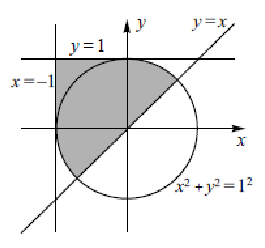
\includegraphics{task2}

\underline{Решение:}

Предлагаем вначале выразить это множество через системы и
совокупности:

$\left[ 
  \begin{gathered} 
    \left\{ 
      \begin{gathered} 
                  x^2 + y^2 \leq 1, \hfill 
        \\ 
        y \geq x \hfill 
        \\ 
      \end{gathered} 
    \right. \hfill 
    \\ 
    \left\{ 
      \begin{gathered} 
                  x^2+y^2 \geq 1, \hfill 
        \\ 
        y \geq 0, \hfill 
        \\ 
        y \leq 1, \hfill 
        \\ 
        x \leq 0, \hfill 
        \\ 
        x \geq -1, \hfill 
        \\ 
      \end{gathered} 
    \right. \hfill 
    \\ 
  \end{gathered} 
\right.$
\\[3pt]

Теперь запишем с использованием характеристического
свойства множества, используя для систем операцию пересечения
множеств, а для совокупности - объединения:

$$X=\{(x;y) \vert x^2+y^2 \leq 1, y \geq x\} \cup \{(x;y)\vert
x^2 + y^2 \geq 1, y \geq 0, y \leq 1, x \leq 0, x \geq -1\}$$

\pagebreak

\textit{\textbf{Задание 3}}

Проиллюстрировать равенство при помощи диаграмм Эйлера-Венна:
$$(A \setminus B) \cup (A \cap C) = A \setminus (B \setminus C)$$

\underline{Решение:}

Построим последовательно левую часть равенства:

\begin{figure}[h]
        \captionsetup[subfigure]{labelformat=empty}
        \centering
        \begin{subfigure}{.32\textwidth}
                \centering
                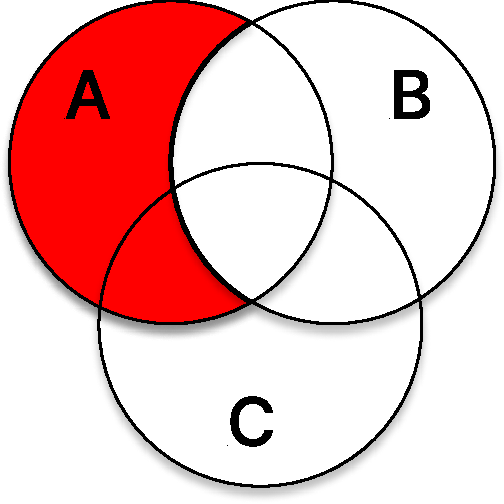
\includegraphics[width=1\linewidth]{t3_1_1.pdf}
                \caption{1. $A \setminus B$}
        \end{subfigure}
        \begin{subfigure}{.32\textwidth}
                \centering
                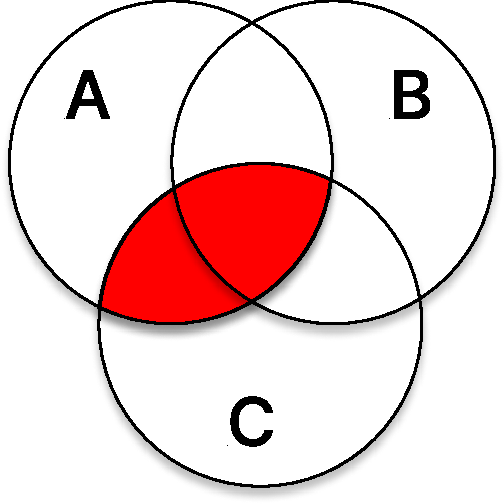
\includegraphics[width=1\linewidth]{t3_1_2.pdf}
                \caption{2. $A\cap C$}
        \end{subfigure}
        \begin{subfigure}{.33\textwidth}
                \centering
                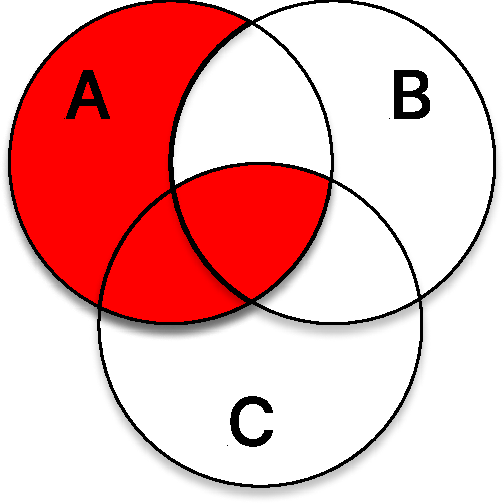
\includegraphics[width=1\linewidth]{t3_1_3.pdf}
                \caption{3. $(A \setminus B) \cup (A \cap C)$}
        \end{subfigure}
\end{figure}

Теперь построим правую часть:

\begin{figure}[h]
        \captionsetup[subfigure]{labelformat=empty}
        \centering
        \begin{subfigure}{.32\textwidth}
                \centering
                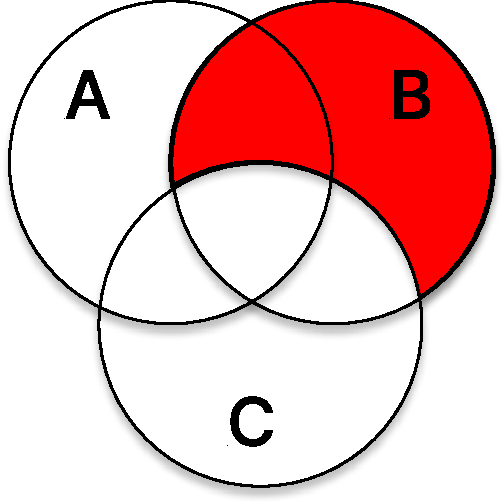
\includegraphics[width=1\linewidth]{t3_2_1.pdf}
                \caption{1. $(B \setminus C)$}
        \end{subfigure}
        \begin{subfigure}{.32\textwidth}
                \centering
                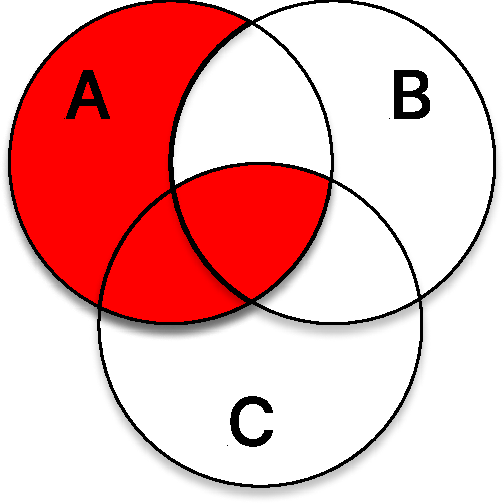
\includegraphics[width=1\linewidth]{t3_2_2.pdf}
                \caption{2. $A \setminus (B \setminus C)$}
        \end{subfigure}
\end{figure}

Диаграммы для левой и правой части оказались одинаковы!

\pagebreak

\textit{\textbf{Задание 4.}}

\textit{Отношение задано матрицей. Исследовать отношение на симметрию,
антисимметрию, асимметрию, рефлексивность, антирефлексивность. Найти
транзитивное замыкание отношения.}

$$M=
\begin{pmatrix}
        0 & 0 & 0 & 1\\
        0 & 1 & 1 & 0\\
        0 & 0 & 1 & 1\\
        0 & 0 & 0 & 1
\end{pmatrix}.$$

\underline{Решение:}

1. Данное отношение не является симметричным, так как матрица
несимметрична. Например, пара (2,3) принадлежит данному отношению, а пара
(3,2) ему не принадлежит.

2. Отношение антисимметрично, так как нет ни одной пары\\
$m_{ij} = m_{ji} = 1, i \neq j$.

3. Отношение антисимметрично, но не асимметрично, так как на
диагонали матрицы имеются элементы равные 1.

4. Не все диагональные элементы метрицы равняются 1.
Данное отношение не является рефлексивным

5. Отношение не обладает свойством антирефлексивности, так как
не все диагональные элементы являются нулевыми

Найдем транзитивное замыкание данного отношения по алгоритму
Уоршолла:

Рассматриваем все внедиагональные $(i \neq j)$ элементы матрицы.
Если $m_{ij}=1$, то $i$-ю строку заменяем дизъюнкцией $i$-й и $j$-й строк.

1. Элемент $m_{14}=1$. Первую строку заменяем поэлементной
дизъюнкцией первой и четвертой строки:

$$M_1=
\begin{pmatrix}
        0 & 0 & 0 & 1\\
        0 & 1 & 1 & 0\\
        0 & 0 & 1 & 1\\
        0 & 0 & 0 & 1
\end{pmatrix}.$$

Данное отношение не является транзитивным, так как, например, пары
(1,2) и (2,4) не принадлежат данному отношению, а пара (1,4)
ему принадлежит.

2. Элемент $m_{23} = 1$. Вторую строку заменяем поэлементной
дизъюнкцией второй и третьей строки:

$$M_2=
\begin{pmatrix}
        0 & 0 & 0 & 1\\
        0 & 1 & 1 & 1\\
        0 & 0 & 1 & 1\\
        0 & 0 & 0 & 1
\end{pmatrix}.$$

3. Элемент $m_{34} = 1}. Дизъюнкция третьей и четвертой строки не меняет
вид матрицы. Таким образом, полученная матрица $M_2$ является матрицей
транзитивного замыкания нашего отношения
\\[10pt]

\textit{\textbf{Задание 5.}}

На множестве упорядоченных пар $x_0=(0,0), x_1=(1,0), x_2=(0,1),\\
x_3=(1,1)$ задана бинарная мультипликативная операция. Произведение задано
по правилу $A*B=(a_2b_2, a_1b_2)$. Является ли полугруппой структура
 $(X,*)$, где $X=\{x_0, x_1, x_2, x_3\}$? Составить таблицу Кэли структуры.

 \underline{Решение:}

Проверим ассоциативность введенного произведения — необходимое
свойство для того, чтобы алгебраическая структура была полугруппой.
Рассмотрим произведение $A*(B*C)$ трёх произвольных пар из X:

$$A=(a_1, a_2), B=(b_1, b_2), C=(c_1, c_2).$$

Найдём сначала произведение $B*C=(b_2c_2, b_1c_2)$, затем получим
$A*(B*C)=(a_2b_1c_2, a_1b_1c_2).$

Аналогично:

$$(A*B)*C=(a_2b_2,a_1b_2)*(c_1,c_2)=(a_1b_2c_2,a_2b_2c_2)$$

Очевидно, $A*(B*C) \neq (A*B)*C$, т.е. операция умножения не ассоциативна
и алгебраическая структура $(X, *)$ не является полугруппой. Составим таблицу Кэли.

\begin{center}
        \begin{tabular}{ |c|c|c|c|c| }
                \hline
                $*$ & $x_0$ & $x_1$ & $x_2$ & $x_3$\\
                \hline
                $x_0$ & $x_0$ & $x_0$ & $x_0$ & $x_0$\\
                \hline
                $x_1$ & $x_0$ & $x_0$ & $x_2$ & $x_2$\\
                \hline
                $x_2$ & $x_0$ & $x_0$ & $x_1$ & $x_1$\\
                \hline
                $x_3$ & $x_0$ & $x_0$ & $x_3$ & $x_3$\\
                \hline
        \end{tabular}
\end{center}

\pagebreak

\textit{\textbf{Задание 6:}}

Построив соответствующую таблицу значений, выясните, равны ли
следующие булевы функции

$$f(x,y,z)=xy' \lor x'y \lor x'z',
\ g(x,y,z)=(x' \lor y')(x \lor y \lor z')$$

\underline{Решение:}

Построим таблицы значений для функций $f$ и $g$:

$$f(x,y,z)=x y' \lor x' y \lor x'z'$$

\begin{center}
        \begin{tabular}{ |c|c|c|c|c|c|c|c|c|c|c| }
                \hline
                $x$ & $y$ & $z$ & $x'$ & $y'$ & $z'$ & $xy'$ & $x'y$ & $x' z'$ & $f(x,y,z)$\\
                \hline
                0 & 0 & 0 & 1 & 1 & 1 & 0 & 0 & 1 & 1\\
                \hline
                0 & 0 & 1 & 1 & 1 & 0 & 0 & 0 & 0 & 0\\
                \hline
                0 & 1 & 0 & 1 & 0 & 1 & 0 & 1 & 1 & 1\\
                \hline
                0 & 1 & 1 & 1 & 0 & 0 & 0 & 1 & 0 & 1\\
                \hline
                1 & 0 & 0 & 0 & 1 & 1 & 1 & 0 & 0 & 1\\
                \hline
                1 & 0 & 1 & 0 & 1 & 0 & 1 & 0 & 0 & 1\\
                \hline
                1 & 1 & 0 & 0 & 0 & 1 & 0 & 0 & 0 & 0\\
                \hline
                1 & 1 & 1 & 0 & 0 & 0 & 0 & 0 & 0 & 0\\
                \hline
        \end{tabular}
\end{center}

$$g(x,y,z)=(x' \lor y')(x \lor y \lor z')$$

\begin{center}
        \begin{tabular}{ |c|c|c|c|c|c|c|c|c| }
                \hline
                $x$ & $y$ & $z$ & $x'$ & $y'$ & $z'$ & $x' \lor y'$ & $x \lor y \lor z'$ & $g(x,y,z)$\\
                \hline
                0 & 0 & 0 & 1 & 1 & 1 & 1 & 1 & 1\\
                \hline
                0 & 0 & 1 & 1 & 1 & 0 & 1 & 0 & 0\\
                \hline
                0 & 1 & 0 & 1 & 0 & 1 & 1 & 1 & 1\\
                \hline
                0 & 1 & 1 & 1 & 0 & 0 & 1 & 1 & 1\\
                \hline
                1 & 0 & 0 & 0 & 1 & 1 & 1 & 1 & 1\\
                \hline
                1 & 0 & 1 & 0 & 1 & 0 & 1 & 1 & 1\\
                \hline
                1 & 1 & 0 & 0 & 0 & 1 & 0 & 1 & 0\\
                \hline
                1 & 1 & 1 & 0 & 0 & 0 & 0 & 1 & 0\\
                \hline
        \end{tabular}
\end{center}

Получили:\\
$$f(x,y,z)=g(x,y,z)$$

\pagebreak

\textit{\textbf{Задание 7:}}

\textit{Постройте минимальную ДНФ для функции тремя разными
способами (графическим способом, картами Карно, методом Квайна):}\\
$f=10111010$

\underline{Решение:}

В данной функции восемь бит, т.е. это функция трех переменных. Будем
считать этими переменными $x$, $y$ и $z$.
В данной функции нулей меньше, поэтому быстрее через них. Разряды:

$$\overset{0}{1} \overset{1}{0} \overset{2}{1} \overset{3}{1} \overset{4}{1} \overset{5}{0} \overset{6}{1} \overset{7}{0}$

тогда нулям соответствуют наборы переменных 001, 101 и 111, а все остальные
наборы – это единицы.

Минимизация графическим способом (метод гиперкубов)

Нарисуем единичный куб в системе координат и выделим его вершины,
координаты которых соответствуют наборам переменных, на которых наша
функция принимает значения 1, и выколем те вершины, которые соответствуют
наборам, на которых принимается значение 0.

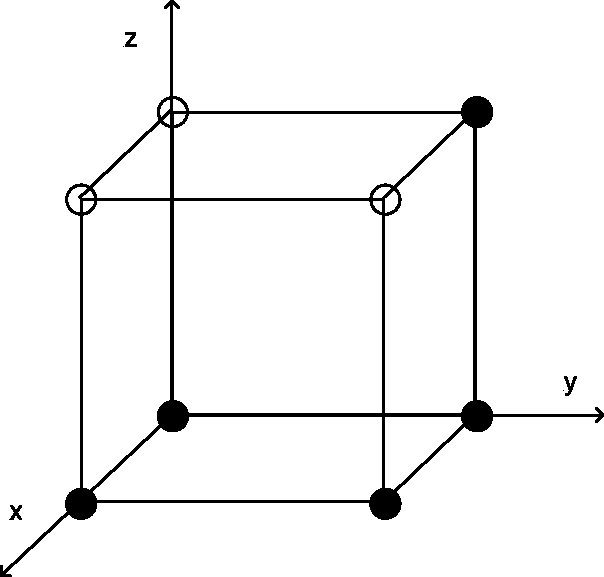
\includegraphics{t7.pdf}

Теперь пробуем покрыть выделенные точки, не зацепив невыделенные
минимальным количеством сначала граней (у нас это не возможно), затем ребер
(у нас все точки покрываются минимально тремя ребрами (выделены на
рисунке ниже), затем, если не удалось ничем ранее, отдельными вершинами.

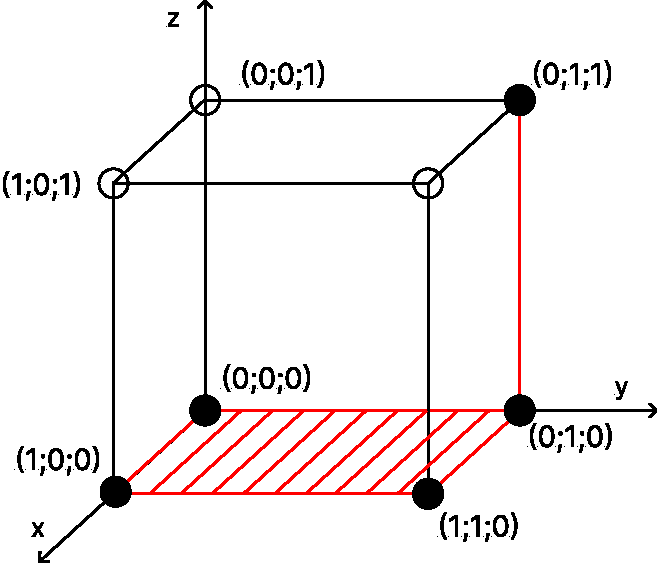
\includegraphics{t7_2.pdf}

Для каждого из выделенных объектов (граней, ребер или вершин)
посмотрим, какие переменные (координаты) не менялись. Для этих переменных
составим конъюнктивные одночлены по правилу построения СДНФ. Например,
для ребра, соединяющего точки с координатами (1;0;0) и (0;0;0) не меняются
вторая (соответствует y) и третья (соответствует z) координаты, и обе они
равны нулю, значит соответствующий конъюнктивный одночлен -y z  , а для
ребра, соединяющего точки (1;0;0) и (1;1;0) не меняются первая и третья
координаты (x и z соответственно), причем x=1, а z=0, тогда получим одночленxz
. Для третьего ребра посмотрите самостоятельно.

\end{document}
